\chapter{Tir oblique}
On appelle \enquote{tir oblique}, \enquote{tir parabolique} ou \enquote{tir balistique}, une situation dans laquelle un objet est lancé vers le haut avec un angle par rapport à l'horizontale. Il s'agit d'un mouvement en deux dimensions, car le mobile se déplace à la fois selon l'axe X et l'axe Y.
\begin{encadre}
    Dans ce mouvement, la position et la vitesse en \(Y\) sont données par les équations du tir vertical. La position et la vitesse en \(X\) sont données par les équations du MRU.
\end{encadre}

\begin{figure}[h!]
    \centering
    %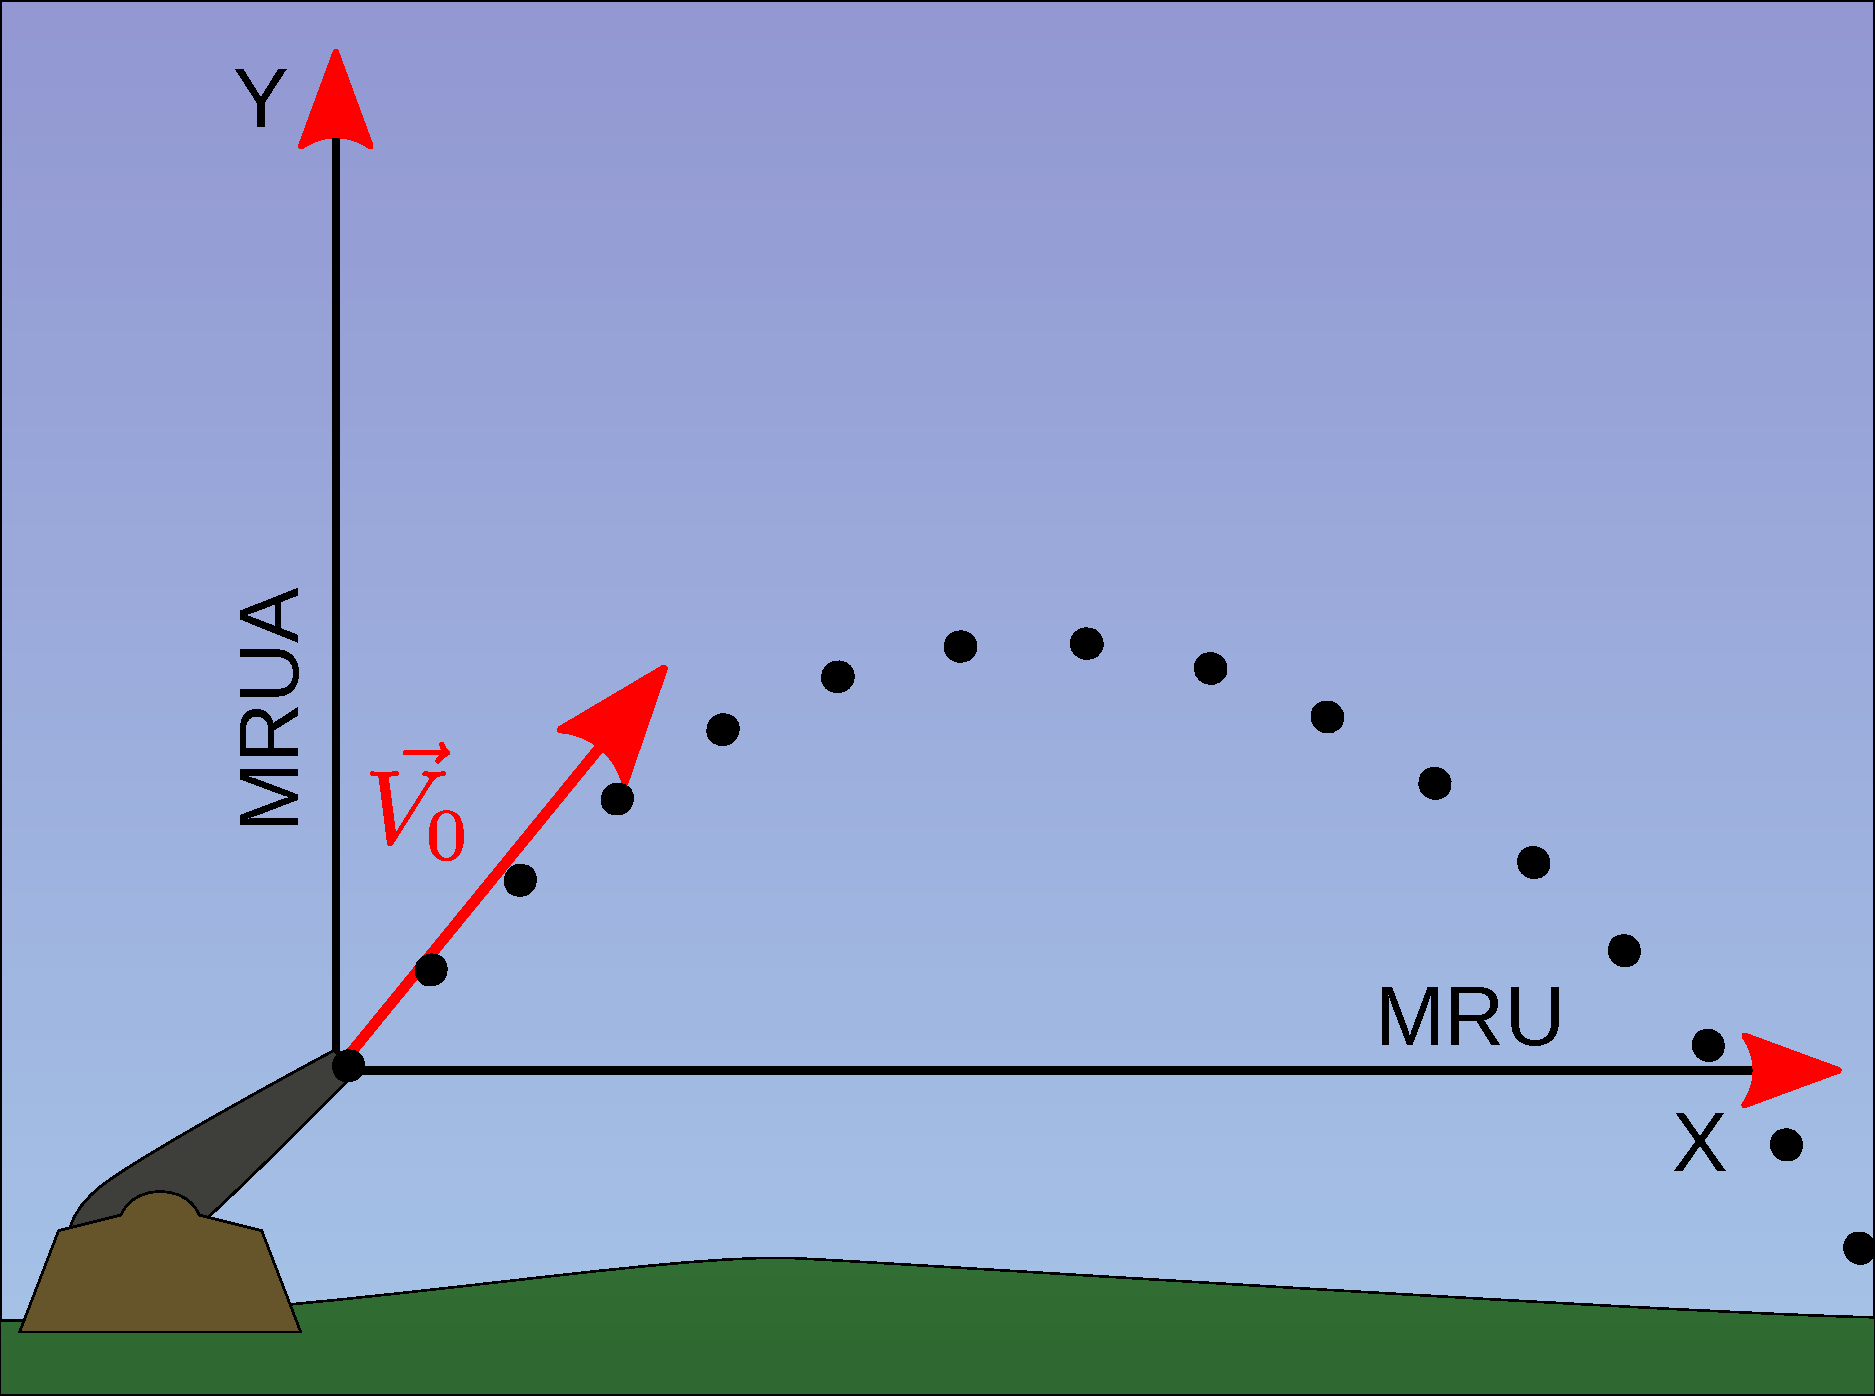
\includegraphics[width=.5 \linewidth]{tir_oblique.pdf}
    \includesvg[inkscapelatex=false, width=.5 \linewidth]{tir_oblique.svg}
    \caption{Schéma d'un tir balistique.}
    \label{Schéma d'un tir balistique}
\end{figure}

\newpage

\section{Caractéristiques du tir oblique}
Comme le montre la chronophotographie ci-dessous, la trajectoire suivie par un objet lancé obliquement est une parabole.

\begin{figure}[h!]
    \centering
    \includegraphics[width=.5 \linewidth]{chronophotographie_tir_oblique.png}
    \caption{Chronophotographie d'un tir parabolique}
    \label{Chronophotographie d'un tir parabolique}
\end{figure}

\section{Décomposition du vecteur vitesse}
La vitesse, comme tout vecteur peut se décomposer en une composante verticale et une composante horizontale. Pour une vitesse \(\vec{v}\) et un angle de tir \(\Theta\), on peut écrire :
\begin{itemize}[label=\textbullet]
    \item \(v_x = v \cdot cos(\theta) \)
    \item \(v_y = v \cdot sin(\theta) \)
\end{itemize}

\begin{tikzpicture}
    %travailler avec euclide au lieu de tkz-base permet d'avoir une description plus explicite du dessin et des emplacements de labels non aribitraire
    \tikzset{>=latex}
    \tkzDefPoint(0,0){o}
    \tkzDefPoint(4,0){a}
    \tkzDefPoint(0,2){b}
    \tkzDefPoint(4,2){c}

    \tkzMarkRightAngle[size=.3,fill=lightgray,opacity=.5](o,a,c)
    \tkzFillAngle[size=1cm,left color=white,right color=YellowOrange](a,o,c)
    \tkzMarkAngle[size = 1cm,color=Orange,mark=none,line width=1pt](a,o,c)
    \tkzLabelAngle[pos=1.25,color=YellowOrange](a,o,c){\(\theta\)}

    \tkzDrawSegment[->,line width=2pt,color=ForestGreen](o,a)
    \tkzLabelSegment[above,color=ForestGreen](o,a){\(\vec{v_x}\)}

    \tkzDrawSegment[->,line width=2pt,color=NavyBlue](o,b)
    \tkzLabelSegment[right,color=NavyBlue](o,b){\(\vec{v_y}\)}

    \tkzDrawSegment[->,line width=2pt,color=Turquoise,style=dashed](a,c)
    \tkzLabelSegment[right,color=Turquoise](a,c){\(\vec{v_y}'\)}

    \tkzDrawSegment[->,line width=2pt,color=BrickRed](o,c)
    \tkzLabelSegment[right=3pt,color=BrickRed](o,c){\(\vec{v_{tot}}\)}
\end{tikzpicture}

\newpage

\section{Calcul du temps d'ascension}
Lors d'un tir oblique avec une vitesse initiale \(\vec{v}\) et un angle de tir \(\theta\), nous savons que :

\begin{itemize}[label=\textbullet]
    \item \(v_x = v \cdot cos(\theta) \)
    \item \(v_y = v \cdot sin(\theta) \)
\end{itemize}

La hauteur maximale est atteinte lorsque  \(v_y(t)=0\). Si \(t_0=0\) alors le temps d'ascension est donné par :

\begin{align}
    v_y(t) & = v_{0y}+a \cdot \Delta t \ \rightarrow \\
    0      & = v_{0y}+a \cdot \Delta t \ \rightarrow \\
    t      & = \frac{-v_{0y}}{a}
\end{align}

Puisque dans un tir oblique \(v_{0y}=v \cdot sin(\theta)\), le temps pris pour atteindre la hauteur maximale est donné par :
\begin{align}
    t = & \frac{-v_{0y}}{a} \ \rightarrow                                             \\
    t = & \tcboxmath[colback=LightBlue,colframe=blue]{\frac{-v \cdot sin(\theta)}{a}}
\end{align}

\newpage

\section{Calcul de la hauteur maximale atteinte}
Lors d'un tir oblique avec une vitesse initiale \(\vec{v}\), un angle de tir \(\theta\) et une hauteur initiale \(y_0\), nous savons que le temps pris pour atteindre la hauteur maximale vaut : \(t=\frac{-v \cdot sin(\theta)}{a}\).

En reprenant l'équation de la position verticale et en remplaçant le temps par celui pris pour atteindre la hauteur maximale et en remplaçant \(v_{0y}\) par \(v \cdot sin(\theta)\), on obtient :

\begin{equation}
    y(t)=y_0 + v_{0y} \cdot t + \frac{a}{2} \cdot t^2
\end{equation} où :

\begin{itemize}[label=\textbullet]
    \item \(t=\frac{-v \cdot sin(\theta)}{a}\)
    \item \(v_{0y}=v \cdot sin(\theta)\)
    \item \(y_0=0\)
\end{itemize}

Donc :

\begin{equation}
    y(t)=v \cdot sin(\theta) \cdot \frac{-v \cdot sin(\theta)}{a} + \frac{a}{2} \frac{v^2 \cdot sin^2(\theta)}{a^2}
\end{equation}

On peut arranger le premier terme puisqu'il y a deux fois les facteurs \enquote{\(v\)} et \enquote{\(sin \theta\)}, on peut aussi simplifier une partie des facteurs \enquote{\(a\)} dans le deuxième terme, cela donne :

\begin{equation}
    y(t)=- \frac{v^2 \cdot sin^2(\theta)}{a} + \frac{1}{2} \frac{v^2 \cdot sin^2(\theta)}{a}
\end{equation}

On peut finalement réduire cette somme pour obtenir :


\begin{equation}
    \tcboxmath[colback=LightBlue,colframe=blue]{y(t)=\frac{-v^2 \cdot sin^2(\theta)}{2 \cdot a}}
\end{equation}

\section{Calcul du temps de chute}
Nous savons que la hauteur maximale atteinte lors du tir oblique est donnée par : \(y(t)=\frac{-v^2 \cdot sin^2(\theta)}{2 \cdot a}\). Quel est alors le temps pris par le mobile pour atteindre le sol depuis cette hauteur ?

Pour cela, il faut utiliser l'équation du mouvement vertical :
\begin{equation}
    y(t)=y_0 + v_{0y} \cdot t + \frac{a}{2} \cdot t^2
\end{equation} où :

\begin{itemize}[label=\textbullet]
    \item \(t_0=0\)
    \item \(v_{0y}=0\)
    \item \(y_t=0\), car on atteint le sol
    \item \(y_0=y_{max}=\frac{-v^2 \cdot sin^2(\theta)}{2 \cdot a}\)
\end{itemize}

Donc :
\begin{align}
    0 & =y_{max}+\frac{a}{2} \cdot t^2 \ \rightarrow     \\
    t & =\sqrt{\frac{-2 \cdot y_{max}}{a}} \ \rightarrow \\
    t & =\sqrt{\frac{v^2 \cdot sin^2 (\theta)}{a^2}}
\end{align}

Il est possible de supprimer la racine carrée, mais n'oublions pas que \(\sqrt{x^2}=\pm x\), donc :
\begin{equation}
    \tcboxmath[colback=LightBlue,colframe=blue]{t=-\frac{v \cdot sin(\theta)}{a}}
\end{equation}

Nous avons pris la racine carrée négative, car \enquote{a} étant négatif, la racine carrée positive n'a pas de sens.

\section{Calcul du temps de parcours total}
La durée de l'ascension et celle de la descente étaient données par : \(\frac{-v \cdot sin(\theta)}{a}\), la durée totale d'un tir oblique vaut donc :

\begin{equation}
    \tcboxmath[colback=LightBlue,colframe=blue]{t_{tot}=\frac{-2 \cdot v \cdot sin(\theta)}{a}}
\end{equation}

\section{Calcul de la distance horizontale parcourue}
Le temps total de parcours lors d'un tir oblique est donné par : \(t_{tot}=\frac{-2 \cdot v \cdot sin(\theta)}{a}\).

La distance parcourue horizontalement est donnée par \(x(t)=x_0+v_x \cdot \Delta t\) où :
\begin{itemize}[label=\textbullet]
    \item \(t_0=0\)
    \item \(x_0=0\)
    \item \(v_x=v \cdot cos(\theta)\)
\end{itemize}

Par conséquent, la distance totale parcourue horizontalement lors d'un tir oblique est donnée par :
\begin{align}
    x(t) & =v \cdot cos(\theta) \cdot \frac{-2 \cdot v \cdot sin(\theta)}{a} \\
    x(t) & =\frac{-2 \cdot v^2 \cdot cos(\theta) \cdot sin(\theta)}{a}
\end{align}

Cette dernière expression peut encore être simplifiée, car elle contient une identité trigonométrique : \(2 \cdot sin(\theta) \cdot cos(\theta)=sin(2 \cdot \theta )\).
Par conséquent :

\begin{equation}
    \tcboxmath[colback=LightBlue,colframe=blue]
    {x(t)=-\frac{v^2 \cdot sin(2 \theta)}{a}}
\end{equation}

\newpage

\section{Exercices}
\begin{exercise}
    Un mobile est lancé depuis le sol avec une vitesse initiale de \(21\unit{[m/s]}\) et avec un angle de \(20^{\circ}\) vers le haut.
    \begin{enumerate}[label=\alph*)]
        \item À quelle distance va-t-il toucher le sol ?
        \item Quelle sera sa vitesse d'impact ?
    \end{enumerate}
\end{exercise}

\begin{exercise}
    Un objet est lancé vers le haut avec une vitesse initiale de \(12\unit{[m/s]}\) et un angle de \(30^{\circ}\) vers le haut.
    \begin{enumerate}
        \item Quelle distance horizontale a-t-il franchi quand il est au sommet de sa course ?
        \item Quelle est sa vitesse totale à ce moment ?
        \item Combien de temps prend-il pour y arriver ?
    \end{enumerate}
\end{exercise}


\begin{exercise}
    Quel doit être l'angle de tir pour toucher un objet situé à une distance de \(127,4[m]\) si la vitesse initiale est de \(50\unit{[m/s]}\) ?
\end{exercise}
\begin{solution}
    \(\theta_1=15^{\circ}\)
    \(\theta_2=75^{\circ}\)
\end{solution}


\begin{exercise}
    Dans un tir oblique, avec quel angle faut-il lancer un objet pour qu'il aille le plus loin possible ?
\end{exercise}
\begin{solution}
    \(\theta=45^{\circ}\)
\end{solution}


\begin{exercise}
    Un objet est lancé avec un angle de \(30^{\circ}\) vers le haut. Quelle doit être sa vitesse initiale pour qu'il touche le sol à \(50[m]\) du lanceur ?
\end{exercise}


\begin{exercise}
    Un objet est lancé avec une vitesse de \(150\unit{[m/s]}\) et un angle de \(70^{\circ}\).
    \begin{enumerate}[label=\alph*)]
        \item Quelle est sa vitesse totale lorsqu'il se trouve à \(50[m]\) horizontalement de son point de départ ?
        \item À quelle hauteur se trouve-t-il ?
    \end{enumerate}
\end{exercise}
\begin{solution}
    \(t_{50}=0,9746[s]\)
    \(v_y=131,4\unit{[m/s]}\)
    \(v_{tot}=141,1\unit{[m/s]}\)
    \(y=132,7[m]\)
\end{solution}


\begin{exercise}
    Un chasseur souhaite tirer une flèche sur un singe situé au sommet d'un arbre de \(50[m]\) de haut et situé à \(30[m]\) de lui. Le chasseur tire sa flèche avec une vitesse de \(20\unit{[m/s]}\) et un angle de \(59^{\circ}\). Au même instant le singe se laisse tomber afin d'éviter la flèche. Montre que le singe aurait mieux fait de rester dans l'arbre !
    \begin{figure}[h!]
        \centering
        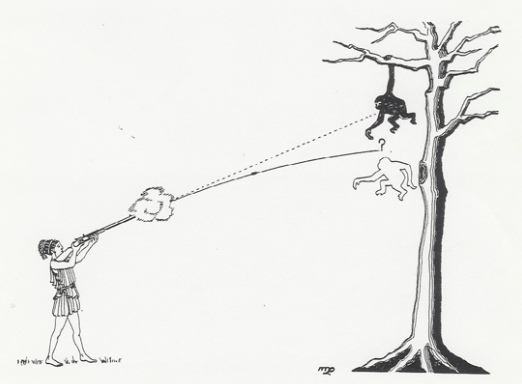
\includegraphics[width=.4 \linewidth]{shoot_monkey.png}
    \end{figure}
\end{exercise}


\begin{exercise}
    Un tigre bondi à l'horizontale du haut d'un rocher de \(16[m]\) à une vitesse de \(6\unit{[m/s]}\). À quelle distance de la base du rocher atterrira-t-il ?
\end{exercise}
\begin{solution}
    \(t=1,8[s] ; x(t)=10,8[m]\)
\end{solution}

\begin{exercise}
    Une lance à incendie tenue près du sol envoie un jet d'eau avec une vitesse de \(13\unit{[m/s]}\). Selon quels angles faut-il l'orienter pour que l'eau retombe \(16[m]\) plus loin ?
\end{exercise}
\begin{solution}
    \(\theta _1 = 34,12 \)
    \(\theta _2 = 55,88 \)
\end{solution}


\begin{exercise}
    En exécutant un saut en longueur un athlète quitte le sol avec un angle de \(28^{\circ}\) et franchit \(8,8[m]\). Détermine sa vitesse lors de l'impulsion.
\end{exercise}
\begin{solution}
    \(v_0=10,204\unit{[m/s]} \)
\end{solution}


\begin{exercise}
    Détermine quelle est la distance supplémentaire franchie par une personne sautant sur la lune par rapport au même saut effectué sur la Terre (même vitesse, même angle). Considère que \(g_{Lune}=\frac{1}{6} g_{Terre}\).
\end{exercise}


\begin{exercise}
    En courant à \(3\unit{[m/s]}\), un plongeur se jette du haut d'une falaise et tombe dans la rivière située en dessous 2 secondes plus tard.
    \begin{enumerate}[label=\alph*)]
        \item Quelle est la hauteur de la falaise ?
        \item À quelle distance de la falaise le plongeur touche-t-il l'eau ?
    \end{enumerate}
\end{exercise}